%%%%%%%%%%%%%%%%%%%%%%%%%%%%%%%%%%%%%%%%%%%%%%
%% Compile: XeLaTeX BibTeX XeLaTeX XeLaTeX
%% Slides: Antonio Machicao y Priemer
%% Course: GK Linguistik
%%%%%%%%%%%%%%%%%%%%%%%%%%%%%%%%%%%%%%%%%%%%%%

%\exewidth{(35)} im übergeordneten File

% sollte zentral geladen werden. St. Mü. 04.11.2016 (in localcommands?)
%%%%%%%%%%%%%
%%% Forestset Syllables

\newbox\foreststrutbox
\setbox\foreststrutbox=\hbox to 0pt{\phantom{\forestOve{standard node}{content}}}
\def\foreststrut{\copy\foreststrutbox}
\forestset{
GP1/.style 2 args={
for n={1}{baseline},
s sep=0pt, l sep=0pt,
for descendants={
l sep=0pt, l={#1},
anchor=base,calign=first,child anchor=north,
inner xsep=1pt,inner ysep=2pt,outer sep=0pt,s sep=0pt,
},
delay={
if content={}{phantom}{for children={no edge}},
for tree={
if content={O}{tier=OR}{},
if content={R}{tier=OR}{},
if content={N}{tier=N}{},
if content={x}{
tier=x,content={$\times$},outer xsep={#2},
for tree={calign=center},
for descendants={content format={\foreststrut\forestoption{content}}},
before drawing tree={outer xsep=0pt,delay={typeset node}},
s sep=4pt
}{},
},
},
before drawing tree={where content={}{parent anchor=center,child anchor=center}{}},
},
GP1/.default={5ex}{8.0pt},
associate/.style={%
tikz+={\draw(!)--(!#1);}},
spread/.style={
before drawing tree={tikz+={\draw[dotted](!)--(!#1);}}},
govern/.style={
before drawing tree={tikz+={\draw[->](!)--(!#1);}}},
p-govern/.style={
before drawing tree={tikz+={\draw[->](.north) to[out=150,in=30] (!#1.north);}}},
no p-govern/.style={
before drawing tree={tikz+={\draw[->,loosely dashed](.north) to[out=150,in=30] (!#1.north);}}},
encircle/.style={before drawing tree={circle,draw,inner sep=0pt}},
fen/.style={pin={[font=\footnotesize,inner sep=1pt,pin edge=<-]10:\textsc{Fen}}},
el/.style={content=\textsc{\textbf{##1}}},
head/.style={content=\textsc{\textbf{\underline{##1}}}},
llap/.style={
tikz+={%
\edef\forest@temp{\noexpand\node[\option{node options},
anchor=base east,at=(.base east)]}%
\forest@temp{#1\phantom{\option{environment}}};
}
},
rlap/.style={
tikz+={%
\edef\forest@temp{\noexpand\node[\option{node options},
anchor=base west,at=(.base west)]}%
\forest@temp{\phantom{\option{environment}}#1};
}
},
}
%%%%%%%%%%%%%


%%%%%%%%%%%%%%%%%%%%%%%%%%%%%%%%%%%%%%%%%%%%%%%%%%%%
%%%             Metadata                         
%%%%%%%%%%%%%%%%%%%%%%%%%%%%%%%%%%%%%%%%%%%%%%%%%%%% 

\title{Grundkurs Linguistik}

\subtitle{Phonologie II: Silbe}

\author[A. Machicao y Priemer]{
	{\small Antonio Machicao y Priemer}
	\\
	{\footnotesize \url{http://www.linguistik.hu-berlin.de/staff/amyp}}
	%	\\
	%	\href{mailto:mapriema@hu-berlin.de}{mapriema@hu-berlin.de}}
}

\institute{Institut für deutsche Sprache und Linguistik}


% bitte lassen, sonst kann man nicht sehen, von wann die PDF-Datei ist.
%\date{ }

%\publishers{\textbf{6. linguistischer Methodenworkshop \\ Humboldt-Universität zu Berlin}}

%\hyphenation{nobreak}


%%%%%%%%%%%%%%%%%%%%%%%%%%%%%%%%%%%%%%%%%%%%%%%%%%%%
%%%             Preamble's End                  
%%%%%%%%%%%%%%%%%%%%%%%%%%%%%%%%%%%%%%%%%%%%%%%%%%%%   


%%%%%%%%%%%%%%%%%%%%%%%%%   
\huberlintitlepage[22pt]
\iftoggle{toc}{
\frame{
%\begin{multicols}{2}
	\frametitle{Inhaltsverzeichnis}
	\tableofcontents
	%[pausesections]
%\end{multicols}
}
}

%%%%%%%%%%%%%%%%%%%%%%%%%%%%%%%%%%
%%%%%%%%%%%%%%%%%%%%%%%%%%%%%%%%%%
%%%%%LITERATURE:

%% Allgemein
\nocite{Glueck&Roedel16a}
\nocite{Schierholz&Co18}
\nocite{Luedeling2009a}
\nocite{Meibauer&Co07a} 
\nocite{Repp&Co15a} 

%%% Sprache & Sprachwissenschaft
%\nocite{Fries16c} %Adäquatheit
%\nocite{Fries16a} %Grammatikalität
%\nocite{Fries&MyP16c} %GG
%\nocite{Fries&MyP16b} %Akzeptabilität
%\nocite{Fries&MyP16d} %Kompetenz vs. Performanz

%% Phonetik & Phonologie
\nocite{Altmann&Co07a}
\nocite{DudenAussprache00a}
\nocite{Hall00a} 
\nocite{Kohler99a}
\nocite{Krech&Co09a}
\nocite{Pompino95a}
\nocite{Ramers08a}
\nocite{Ramers&Vater92a}
\nocite{Rues&Co07a}
\nocite{WieseR96a}
\nocite{WieseR11a}


%%%%%%%%%%%%%%%%%%%%%%%%%%%%%%%%%%
%%%%%%%%%%%%%%%%%%%%%%%%%%%%%%%%%%
\section{Phonologie II: Silbe}
%%%%%%%%%%%%%%%%%%%%%%%%%%%%%%%%%%

%@EE: Checken: Struktur -- Reihenfolge der Folien
%@EE: Checken: Inhaltsverzeichnisse usw.
%@EE: Checken: wenn 3b und 3c stehen, kann der auskommentierte Text am Ende von 3b gelöscht werden

%%%%%%%%%%%%%%%%%%%%%%%%%%%%%%%%%%

\begin{frame}
\frametitle{Begleitlektüre}

\begin{itemize}
	\item \textbf{obligatorisch:}
	\begin{itemize}
		\item[] AM S.~18--23
	\end{itemize}
	\item \textbf{optional:}
	\begin{itemize}
		\item[] \citet{Hall00a}: Kapitel~8 (S.~205--230)
	\end{itemize}
\end{itemize}

\end{frame}


%%%%%%%%%%%%%%%%%%%%%%%%%%%%%%%%%%%%
%%%%%%%%%%%%%%%%%%%%%%%%%%%%%%%%%
\subsection{Einführung}

%% MyP: Contents
\iftoggle{sectoc}{
	\frame{
		%\begin{multicols}{2}
		\frametitle{~}
		\tableofcontents[currentsubsection, subsubsectionstyle=hide]
		%\end{multicols}
	}
}

%% StM: Contents
\iftoggle{gliederung}{
	
	\outline{
		\begin{itemize}
			
			\item \blaubf{Einführung}
			\item Silbenbestimmung
			\item Silbenstruktur
			%% Onset
			%% Nukleus
			%% Koda
			\item Phonotaktik
			%% Sonoritätshierarchie
			%% Weitere phonotaktische Beschränkungen
			\item Hausaufgabe
			
		\end{itemize}
	}
}
%%%%%%%%%%%%%%%%%%%%%%%%%%%%%%%%%%%
\begin{frame}
\frametitle{Einführung: Notation}


\begin{itemize}
	\item graphematische Notation in spitzen Klammern: 
	
	  \ea
          \ab{nordwind}, \ab{Nordwind}
          \z
% zwei Varianten, eine phonographisches Prinzip, eine mit syntaktischer Info = Großschreibung
          
	\item[]	
	\item phonetische Notation in eckigen Klammern:
	
	  \ea
          \textipa{[nO5t.vInt]}
	  \z
          
	\item[]
	\item phonologische Notation in Schrägstrichen:
	
	  \ea
          \textipa{/nO\textscr d.vInd/}
	  \z
\end{itemize}

\end{frame}



%%%%%%%%%%%%%%%%%%%%%%%%%%%%%%%%%%%
\begin{frame}
\frametitle{Silben}

Warum nimmt man Silben an?

\begin{itemize}
	\item Die Auslautverhärtung mit Bezug auf das Wort (vorläufig):
	
	\ea {}[$-$son] $\rightarrow$ [$-$sth] /\_\_ \#
             
	{\small (ein nicht-sonoranter Laut -- d.\,h.\ Obstruent -- wird am Wortende nicht-stimmhaft)}
	\z
     
	\item Transkribieren Sie: (\emph{sie}) \emph{siegte}

% Auslautverhärtung auch bei Silben
\pause	

	\ea
	\textipa{[zi:k . t@]} (\gqq{.} steht für Silbengrenze)
	\z

%\pause
%
%	\eal 
%	\ex \textipa{[St\textscr e:p.za:m]} \vs \textipa{[St\textscr e:.b5]}
%	\ex \textipa{[bYnt.nIs]} \vs \textipa{[bUn.d@s]}
%	\ex \textipa{[bi:k.za:m]} \vs \textipa{[bi:.g@n]}
%	\ex \textipa{[le:s.b5]} \vs \textipa{[le:.z@n]}
%    \zl
%        
%	\item Auslautverhärtung mit Bezug auf die \textbf{Silbe}:
%	  \ea
%             {}[$-$son] $\rightarrow$ [$-$sth] /\_\_ $]_{\sigma}$
%	  \z	
\end{itemize}

\end{frame}


%%%%%%%%%%%%%%%%%%%%%%%%%%%%%%%%%%%
\begin{frame}
\frametitle{Silben}

\begin{itemize}
	\item Vergleichen Sie:

\ea 

\begin{tabular}[t]{lllclll}
\only<1->{a. \ab{stre\alertred{b}sam} & \vs & \ab{Stre\alertred{b}er} &} \only<2->{~ & \textipa{[St\textscr e:\alertred{p}.za:m]} & \vs & \textipa{[St\textscr e:.\alertred{b}5]}}\\

\only<1->{b. \ab{Bün\alertred{d}nis} & \vs & \ab{Bun\alertred{d}es} &} \only<3->{~ & \textipa{[bYn\alertred{t}.nIs]} & \vs & \textipa{[bUn.\alertred{d}@s]}}\\

\only<1->{c. \ab{bie\alertred{g}sam} & \vs & \ab{bie\alertred{g}en} &} \only<4->{& \textipa{[bi:\alertred{k}.za:m]} & \vs &  \textipa{[bi:.\alertred{g}@n]}} \\

\only<1->{d. \ab{le\alertred{s}bar} & \vs & \ab{le\alertred{s}en} &} \only<5->{& \textipa{[le:\alertred{s}.b5]} & \vs &  \textipa{[le:.\alertred{z}@n]}} \\

\end{tabular}

\z 

%\begin{columns}
%\begin{column}[t]{.5\linewidth}
%\eal 
%	\ex \ab{stre\alertred{b}sam} \vs \ab{Stre\alertred{b}er}
%	\ex \ab{Bün\alertred{d}nis} \vs \ab{Bun\alertred{d}es} 
%	\ex \ab{bie\alertred{g}sam} \vs \ab{bie\alertred{g}en}
%	\ex \ab{le\alertred{s}bar} \vs \ab{le\alertred{s}en}
%\zl	
%\end{column}
%
%%\pause 
%
%\begin{column}[t]{\linewidth}
%\begin{itemize}
%%\eal 
%%\ex 
%	\item[] \textipa{[St\textscr e:\alertred{p}.za:m]} \vs \textipa{[St\textscr e:.\alertred{b}5]}
%%\ex 
%	\item[] \textipa{[bYn\alertred{t}.nIs]} \vs \textipa{[bUn.\alertred{d}@s]}
%%\ex 
%	\item[] \textipa{[bi:\alertred{k}.za:m]} \vs \textipa{[bi:.\alertred{g}@n]}
%%\ex 
%	\item[] \textipa{[le:\alertred{s}.b5]} \vs \textipa{[le:.\alertred{z}@n]}
%%\zl
%\end{itemize}
%\end{column}
%
%\end{columns}	
\end{itemize}


\begin{itemize}
	\item<6-> Auslautverhärtung mit Bezug auf die \textbf{Silbe}:
	\ea
	{}[$-$son] $\rightarrow$ [$-$sth] /\_\_ $]_{\sigma}$
	\z	
\end{itemize}

\end{frame}


%%%%%%%%%%%%%%%%%%%%%%%%%%%%%%%%%%%
\begin{frame}
\frametitle{Silben}

Warum nimmt man Silben an?

Silbe als \textbf{Domäne} \ldots

\begin{itemize}	
	\item \ldots\ verschiedener \textbf{phonologischer Prozesse}\\
               (\zB Auslautverhärtung, Knacklauteinsetzung, Aspiration, \ldots )
	
	\item[] 
	
	\item \ldots\ von Regularitäten bzgl. der \textbf{Abfolge} von Lauten
	
	\item[]
	
	\item \ldots\ der \textbf{Wortbetonung}, d.\,h. wichtige so genannte prosodische Einheiten (Prosodie $=$ Betonung mit Bezug auf Einheiten über dem Segment)
\end{itemize}

\end{frame}



%%%%%%%%%%%%%%%%%%%%%%%%%%%%%%%%%%%
%
%\begin{frame}
%\frametitle{Prosodische Konstituenten}
%
%
%	\begin{multicols}{2}
%	\begin{itemize*}
%		\item UP = Äußerungsphrase
%		\item IP = Intonationsphrase
%		\item $\phi$ = phonol. Phrase
%\columnbreak
%		\item $\omega$ = phonol. Wort
%		\item F = phonol. Fuß
%		\item \alertred{$\sigma$ = Silbe}
%	\end{itemize*}
%	\end{multicols}
%
%\begin{figure} %%rote Box einfügen
%	\centering
%	\scalebox{.68}{
%	\begin{forest} MyP edges,
%	[IP
%	[$\Phi$
%	[$\omega$[F[\alertred{$\sigma$}[Frau]]]]
%	[$\omega$[F[\alertred{$\sigma$}[Müll, name=mueller]][\alertred{$\sigma$}, name=sigma[er]]]]]
%	[$\Phi$
%	[$\omega$[F[\alertred{$\sigma$}[kauft]]]]
%	[$\omega$[F[\alertred{$\sigma$}[Steck]]]
%			 [F[\alertred{$\sigma$}[rü]]
%			   [\alertred{$\sigma$}[ben]]]]]
%	[$\Phi$
%	[$\omega$[F[\alertred{$\sigma$}[auf]]]
%			 [F[\alertred{$\sigma$}[dem]]]]
%	[$\omega$[F[\alertred{$\sigma$}[Woch, name=woch]]
%			   [\alertred{$\sigma$}, name=sigmab[en]]]
%			 [F[\alertred{$\sigma$}[markt]]]]]
%	]
%	{
%		\draw[black] (mueller.north)--(sigma.south);
%		\draw[black] (woch.north)--(sigmab.south);
%	}
%	\end{forest}
%}
%	\caption{nach C. Féry}
%	\label{Zeichen1}
%\end{figure}
%
%% Doppeltverwendung bei Silbengelenken Mül ler
%
%% betonte Silben bilden Fuß einschließlich allen folgenden unbetonten Silben
%
%%\begin{figure}[b]
%%	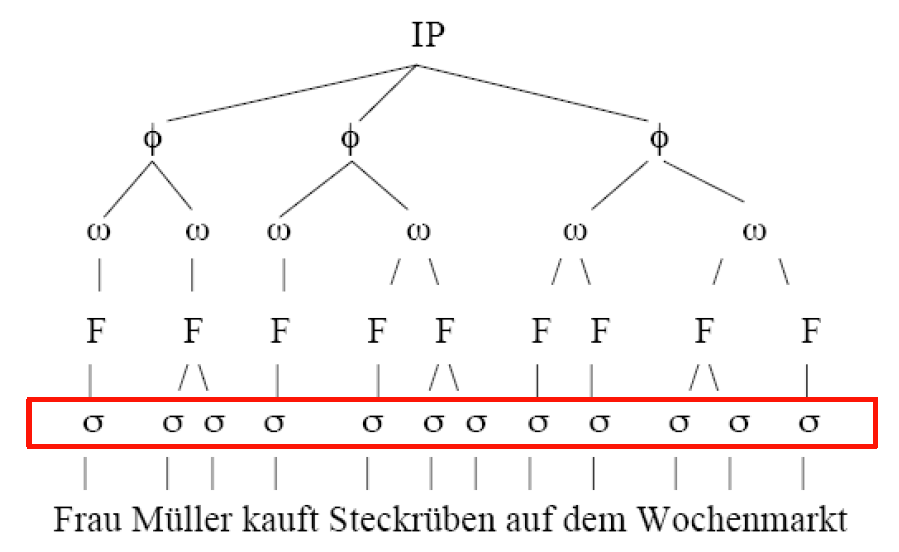
\includegraphics[scale=0.3]{material/03bHierarchieIntonationsphrase}
%%	\caption{Hierarchie in der Intonationsphrase (Darstellung von C. Féry)}
%%	\label{Zeichen1}
%%\end{figure}
%
%\end{frame}

%%%%%%%%%%%%%%%%%%%%%%%%%%%%%%%%%%%
\begin{frame}
\frametitle{Prosodische Konstituenten}

	\begin{multicols}{2}
	\begin{itemize*}
		\item UP = Äußerungsphrase
		\item IP = Intonationsphrase
		\item $\varphi$ = phonol. Phrase
\columnbreak
		\item $\omega$ = phonol. Wort
		\item F = phonol. Fuß
		\item \alertred{$\sigma$ = Silbe}
	\end{itemize*}
	\end{multicols}


	\begin{figure}
	\centering
	\scalebox{.68}{
		\begin{forest} MyP edges,
		[UP, name=up
		[IP, name=IP
		[$\varphi$[$\omega$[F[$\sigma$][$\sigma$]][F[$\sigma$][$\sigma$]]]]
		[$\varphi$, name=Phi[$\omega$[F[$\sigma$][$\sigma$]]][$\omega$, name=omega[F, name=F[$\sigma$][$\sigma$, name=sigma]]]]
		]]
		{\draw[black] (up.east)--(3,0);
			\draw[black] (IP.east)--(3,-1);
			\draw[black] (Phi.east)--(3,-2);
			\draw[black] (omega.east)--(3,-3);
			\draw[black] (F.east)--(3,-4);
			\draw[black] (sigma.east)--(3,-5.3);
			\node[right] at (3,0) {(Mandarinen oder Äpfel)\textsubscript{UP}};
			\node[right] at (3,-1) {(Mandarinen oder Äpfel)\textsubscript{IP}};
			\node[right] at (3,-2) {(Mandarinen)\textsubscript{$\varphi$} (oder Äpfel)\textsubscript{$\varphi$}};
			\node[right] at (3,-3) {(Mandarinen)\textsubscript{$\omega$} (oder)\textsubscript{$\omega$} (Äpfel)\textsubscript{$\omega$}};
			\node[right] at (3,-4) {(Manda)\textsubscript{F} (rinen)\textsubscript{F} (oder)\textsubscript{F} (Äpfel)\textsubscript{F}};
			\node[right] at (3,-5.3) {(Man)\textsubscript{$\sigma$} (da)\textsubscript{$\sigma$} (ri)\textsubscript{$\sigma$} (nen)\textsubscript{$\sigma$} (o)\textsubscript{$\sigma$} (der)\textsubscript{$\sigma$} (Äp)\textsubscript{$\sigma$} (fel)\textsubscript{$\sigma$}};
	}
		\end{forest}
	}
		\caption{\cite{Fuhrhop&Co13a}}
	\end{figure}

%\begin{figure}[b]
%	\centering
%	
%	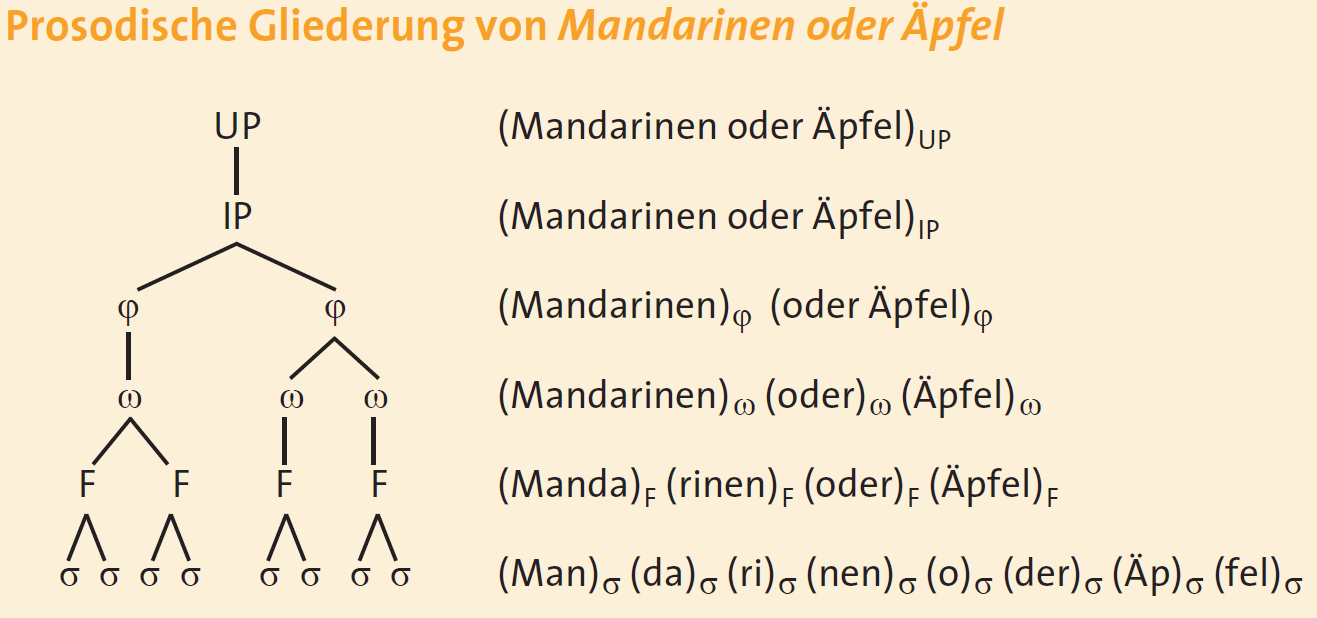
\includegraphics[scale=0.26]{material/03bHierarchieUP}
%	\caption{Hierarchie in der Äußerungsphrase \citep[8]{Fuhrhop&Co13a}}
%	%\label{Zeichen1}
%\end{figure}

\end{frame}


%%%%%%%%%%%%%%%%%%%%%%%%%%%%%%%%%%
%%%%%%%%%%%%%%%%%%%%%%%%%%%%%%%%%%
\subsection{Silbenbestimmung}

%% MyP: Contents
\iftoggle{sectoc}{
	\frame{
		%\begin{multicols}{2}
		\frametitle{~}
		\tableofcontents[currentsubsection, subsubsectionstyle=hide]
		%\end{multicols}
	}
}

%% StM: Contents
\iftoggle{gliederung}{
	
	\outline{
		\begin{itemize}
			
			\item Einführung
			\item \blaubf{Silbenbestimmung}
			\item Silbenstruktur
			%% Onset
			%% Nukleus
			%% Koda
			\item Phonotaktik
			%% Sonoritätshierarchie
			%% Weitere phonotaktische Beschränkungen
			\item Hausaufgabe
			
		\end{itemize}
	}
}
%%%%%%%%%%%%%%%%%%%%%%%%%%%%%%%%%%

\begin{frame}
\frametitle{Silbenbestimmung}

\begin{itemize}
	\item<1-> Wie viele Silben hat das folgende Wort?
	
	\ea Silbenbestimmung
	\z
	
	\item<2-> Woher wissen Sie das?
	
	\begin{itemize}
		\item[]<2-> \gqq{Jeder kompetente Sprachteilhaber verfügt über die \textbf{Fähigkeit},\\
 Silben identifizieren zu können.}  \citep[133]{Staffeldt10a}

		\vspace{.25cm}

		\item[]<2-> \gqq{Silbe: Phonetisch-phonologische \textbf{Grundeinheit} des Wortes
                  bzw.\ der Rede, die zwar \textbf{intuitiv} nachweisbar ist, wissenschaftlich aber \textbf{nicht einheitlich definiert} wird.} \citep[600]{Bussmann02a}
		
	\end{itemize}
 
	\item<3-> Silben können \textbf{betont} werden (tragen Akzent)
	
	\item<4-> \textbf{Silbenspiele} (\zB \only<5->{Sil\alertred{pi}-ben\alertred{pe}-spie\alertred{pi}-le\alertred{pe},} \only<5->{Si\alertred{hi}l-be\alertred{he}n-spie\alertred{hi}-le\alertred{he})}
% Geheimsprache, nach Silben wird immer pi, pa, pe oder so eingesetzt
	
	\item<6-> \textbf{Intuitiv} erkennbare Einheit: 
	
	Kinder können in einem sehr frühen Alter intuitiv Silben klatschen.

\end{itemize}

\end{frame}



%%%%%%%%%%%%%%%%%%%%%%%%%%%%%%%%%%
%%%%%%%%%%%%%%%%%%%%%%%%%%%%%%%%%%
\subsection{Silbenstruktur}

%% MyP: Contents
\iftoggle{sectoc}{
	\frame{
		%\begin{multicols}{2}
		\frametitle{~}
		\tableofcontents[currentsubsection, subsubsectionstyle=hide]
		%\end{multicols}
	}
}

%% StM: Contents
\iftoggle{gliederung}{
	
	\outline{
		\begin{itemize}
			
			\item Einführung
			\item Silbenbestimmung
			\item \blaubf{Silbenstruktur}
			%% Onset
			%% Nukleus
			%% Koda
			\item Phonotaktik
			%% Sonoritätshierarchie
			%% Weitere phonotaktische Beschränkungen
			\item Hausaufgabe
			
		\end{itemize}
	}
}
%%%%%%%%%%%%%%%%%%%%%%%%%%%%%%%%%%
\begin{frame}
\frametitle{Silbenstruktur}

\begin{itemize}
	\item Welche Silben (des Deutschen) sind mit den folgenden Segmenten bildbar?

\ea \textipa{[p]}, \textipa{[a]}, \textipa{[l]}, \textipa{[t]}
\z

\pause	

\begin{multicols}{2}
\ea \textbf{bildbar:}\\
	\textipa{[palt]},\\
	\textipa{[alpt]}, \\
	\textipa{[lapt]}, \\
	\textipa{[talp]}, \\
	\textipa{[plat]}
\z 

\columnbreak

\pause

	\ea \textbf{nicht bildbar:}\\
	*\textipa{[ltap]}, \\
	*\textipa{[lpat]},\\
	*\textipa{[ptla]}, \\
	*\textipa{[tpal]}, 	\ldots 
\z
\end{multicols}

\pause

\item Warum?

\end{itemize}

\end{frame}



%%%%%%%%%%%%%%%%%%%%%%%%%%%%%%%%%%%
%\begin{frame}
%\frametitle{Silbenstruktur}
%
%Die Silbe ist \textbf{intern strukturiert} und besteht aus den folgenden Teilen:
%
%\begin{minipage}{.60\textwidth}
%
%\begin{itemize}
%	\item[]
%	\item Silbenanlaut/Silbenanfangsrand/\alert{Onset},
%	\begin{itemize}
%		\item 0 bis $n$ Konsonanten, wobei in fast allen Sprachen $n < 5$
%	\end{itemize}
%	
%	\item[]
%	\item Silbengipfel/Silbenkern/\alert{Nukleus},
%	\begin{itemize}
%		\item Vokale
%		\item manchmal (vokalische) Nasale oder Liquide
%	\end{itemize}
%	
%	\item[]
%	\item Silbenauslaut/Silbenendrand/\alert{Koda}
%	\begin{itemize}
%		\item 0 bis $n$ Konsonanten, wobei in fast allen Sprachen $n < 5$
%	\end{itemize}
%
%	\item[]
%	\item Nukleus und Koda bilden den \alert{Reim}
%	
%\end{itemize}
%
%
%\end{minipage}
%\begin{minipage}{.39\textwidth}
%
%%%%%%%%%%%%%%
%%% Forestset Syllables

\newbox\foreststrutbox
\setbox\foreststrutbox=\hbox to 0pt{\phantom{\forestOve{standard node}{content}}}
\def\foreststrut{\copy\foreststrutbox}
\forestset{
GP1/.style 2 args={
for n={1}{baseline},
s sep=0pt, l sep=0pt,
for descendants={
l sep=0pt, l={#1},
anchor=base,calign=first,child anchor=north,
inner xsep=1pt,inner ysep=2pt,outer sep=0pt,s sep=0pt,
},
delay={
if content={}{phantom}{for children={no edge}},
for tree={
if content={O}{tier=OR}{},
if content={R}{tier=OR}{},
if content={N}{tier=N}{},
if content={x}{
tier=x,content={$\times$},outer xsep={#2},
for tree={calign=center},
for descendants={content format={\foreststrut\forestoption{content}}},
before drawing tree={outer xsep=0pt,delay={typeset node}},
s sep=4pt
}{},
},
},
before drawing tree={where content={}{parent anchor=center,child anchor=center}{}},
},
GP1/.default={5ex}{8.0pt},
associate/.style={%
tikz+={\draw(!)--(!#1);}},
spread/.style={
before drawing tree={tikz+={\draw[dotted](!)--(!#1);}}},
govern/.style={
before drawing tree={tikz+={\draw[->](!)--(!#1);}}},
p-govern/.style={
before drawing tree={tikz+={\draw[->](.north) to[out=150,in=30] (!#1.north);}}},
no p-govern/.style={
before drawing tree={tikz+={\draw[->,loosely dashed](.north) to[out=150,in=30] (!#1.north);}}},
encircle/.style={before drawing tree={circle,draw,inner sep=0pt}},
fen/.style={pin={[font=\footnotesize,inner sep=1pt,pin edge=<-]10:\textsc{Fen}}},
el/.style={content=\textsc{\textbf{##1}}},
head/.style={content=\textsc{\textbf{\underline{##1}}}},
llap/.style={
tikz+={%
\edef\forest@temp{\noexpand\node[\option{node options},
anchor=base east,at=(.base east)]}%
\forest@temp{#1\phantom{\option{environment}}};
}
},
rlap/.style={
tikz+={%
\edef\forest@temp{\noexpand\node[\option{node options},
anchor=base west,at=(.base west)]}%
\forest@temp{\phantom{\option{environment}}#1};
}
},
}
%%%%%%%%%%%%%

%\begin{figure}
%\centering
%\begin{forest} MyP edges, GP1 [
%  [$\sigma$
%    [O	[ [C$^{n}$]]
%    ]
%    [R	[N
%    		[V$^{n}$]
%    	]
%    	[K
%    		[C$^{n}$]
%    	]
%    ]
%  ]
%]
%\end{forest}
%\caption{Silbenstruktur}
%\end{figure}
%
%\end{minipage}
%
%\end{frame}



%%%%%%%%%%%%%%%%%%%%%%%%%%%%%%%%%%

\begin{frame}
\frametitle{Silbenstruktur: komplexe Silbe}

Die Silbe ist \textbf{intern strukturiert} und besteht aus den folgenden Teilen:

\begin{minipage}{.59\textwidth}

\begin{itemize}
	\item[]
	\item \alertred{Onset} 
	
	\item \alertred{Reim} 
	
	\item \alertred{Nukleus}
	
	\item \alertred{Koda}
	\item[] 
	\item C $:=$ konsonantisch, d.\,h. nicht-silbisch ($\neq$Konsonant)
	
	\item V $:=$ vokalisch, d.\,h. silbisch ($\neq$Vokal)
	
\end{itemize}


\end{minipage}
\begin{minipage}{.40\textwidth}

%%%%%%%%%%%%%%
%%% Forestset Syllables

\newbox\foreststrutbox
\setbox\foreststrutbox=\hbox to 0pt{\phantom{\forestOve{standard node}{content}}}
\def\foreststrut{\copy\foreststrutbox}
\forestset{
GP1/.style 2 args={
for n={1}{baseline},
s sep=0pt, l sep=0pt,
for descendants={
l sep=0pt, l={#1},
anchor=base,calign=first,child anchor=north,
inner xsep=1pt,inner ysep=2pt,outer sep=0pt,s sep=0pt,
},
delay={
if content={}{phantom}{for children={no edge}},
for tree={
if content={O}{tier=OR}{},
if content={R}{tier=OR}{},
if content={N}{tier=N}{},
if content={x}{
tier=x,content={$\times$},outer xsep={#2},
for tree={calign=center},
for descendants={content format={\foreststrut\forestoption{content}}},
before drawing tree={outer xsep=0pt,delay={typeset node}},
s sep=4pt
}{},
},
},
before drawing tree={where content={}{parent anchor=center,child anchor=center}{}},
},
GP1/.default={5ex}{8.0pt},
associate/.style={%
tikz+={\draw(!)--(!#1);}},
spread/.style={
before drawing tree={tikz+={\draw[dotted](!)--(!#1);}}},
govern/.style={
before drawing tree={tikz+={\draw[->](!)--(!#1);}}},
p-govern/.style={
before drawing tree={tikz+={\draw[->](.north) to[out=150,in=30] (!#1.north);}}},
no p-govern/.style={
before drawing tree={tikz+={\draw[->,loosely dashed](.north) to[out=150,in=30] (!#1.north);}}},
encircle/.style={before drawing tree={circle,draw,inner sep=0pt}},
fen/.style={pin={[font=\footnotesize,inner sep=1pt,pin edge=<-]10:\textsc{Fen}}},
el/.style={content=\textsc{\textbf{##1}}},
head/.style={content=\textsc{\textbf{\underline{##1}}}},
llap/.style={
tikz+={%
\edef\forest@temp{\noexpand\node[\option{node options},
anchor=base east,at=(.base east)]}%
\forest@temp{#1\phantom{\option{environment}}};
}
},
rlap/.style={
tikz+={%
\edef\forest@temp{\noexpand\node[\option{node options},
anchor=base west,at=(.base west)]}%
\forest@temp{\phantom{\option{environment}}#1};
}
},
}
%%%%%%%%%%%%%


\begin{figure}
\centering
\begin{forest} MyP edges, GP1 [
  [$\sigma$
    [O
    	[[C[\textipa{S}]]]
    	[[C[\textipa{t}]]]
    	[[C[\textipa{\textscr}]]]
    ]
    [R
    	[N
    		[V[\textipa{U}]]
    	]
    	[K
    		[C[\textipa{m}]]
    		[C[\textipa{\t{pf}}]]
    		[C[\textipa{s}]]
    		[C[\textipa{t}]]
    	]
    ]
  ]
]
\end{forest}
%\caption{Komplexe Silbe}
\end{figure}
% wahrscheinlich komplexeste Koda, die es gibt.
\end{minipage}

\end{frame}


%%%%%%%%%%%%%%%%%%%%%%%%%%%%%%%%%%
\begin{frame}
\frametitle{Silbenstruktur: minimale Silbe}

Die Silbe ist \textbf{intern strukturiert} und besteht aus den folgenden Teilen:

\begin{minipage}{.60\textwidth}

\begin{itemize}
	\item[]
	\item \alertred{Onset}
	
	\item \alertred{Reim}
	
	\item \alertred{Nukleus}
	
	\item \alertred{Koda}
	\item[] 
	\item \textbf{Minimale Silbe} besteht nur aus einem V im  Nukleus
	  \ea
          \ab{gehe} \ras \textipa{[ge:.\alertred{@}]}
          \z
	
\end{itemize}


\end{minipage}
\begin{minipage}{.39\textwidth}

%%%%%%%%%%%%%%
%%% Forestset Syllables

\newbox\foreststrutbox
\setbox\foreststrutbox=\hbox to 0pt{\phantom{\forestOve{standard node}{content}}}
\def\foreststrut{\copy\foreststrutbox}
\forestset{
GP1/.style 2 args={
for n={1}{baseline},
s sep=0pt, l sep=0pt,
for descendants={
l sep=0pt, l={#1},
anchor=base,calign=first,child anchor=north,
inner xsep=1pt,inner ysep=2pt,outer sep=0pt,s sep=0pt,
},
delay={
if content={}{phantom}{for children={no edge}},
for tree={
if content={O}{tier=OR}{},
if content={R}{tier=OR}{},
if content={N}{tier=N}{},
if content={x}{
tier=x,content={$\times$},outer xsep={#2},
for tree={calign=center},
for descendants={content format={\foreststrut\forestoption{content}}},
before drawing tree={outer xsep=0pt,delay={typeset node}},
s sep=4pt
}{},
},
},
before drawing tree={where content={}{parent anchor=center,child anchor=center}{}},
},
GP1/.default={5ex}{8.0pt},
associate/.style={%
tikz+={\draw(!)--(!#1);}},
spread/.style={
before drawing tree={tikz+={\draw[dotted](!)--(!#1);}}},
govern/.style={
before drawing tree={tikz+={\draw[->](!)--(!#1);}}},
p-govern/.style={
before drawing tree={tikz+={\draw[->](.north) to[out=150,in=30] (!#1.north);}}},
no p-govern/.style={
before drawing tree={tikz+={\draw[->,loosely dashed](.north) to[out=150,in=30] (!#1.north);}}},
encircle/.style={before drawing tree={circle,draw,inner sep=0pt}},
fen/.style={pin={[font=\footnotesize,inner sep=1pt,pin edge=<-]10:\textsc{Fen}}},
el/.style={content=\textsc{\textbf{##1}}},
head/.style={content=\textsc{\textbf{\underline{##1}}}},
llap/.style={
tikz+={%
\edef\forest@temp{\noexpand\node[\option{node options},
anchor=base east,at=(.base east)]}%
\forest@temp{#1\phantom{\option{environment}}};
}
},
rlap/.style={
tikz+={%
\edef\forest@temp{\noexpand\node[\option{node options},
anchor=base west,at=(.base west)]}%
\forest@temp{\phantom{\option{environment}}#1};
}
},
}
%%%%%%%%%%%%%


\begin{figure}
\centering
\begin{forest} MyP edges, GP1 [
  [$\sigma$
    [O
    ]
    [R
    	[N
    		[V[\textipa{@}]]
    	]
    	[K
    	]
    ]
  ]
]
\end{forest}
%\caption{Minimale Silbe}
\end{figure}


\end{minipage}

\end{frame}


%%%%%%%%%%%%%%%%%%%%%%%%%%%%%%%%%%
\begin{frame}
\frametitle{Offene/geschlossene/nackte/bedeckte Silben}

\begin{itemize}
	\item Silbenanlaut/Silbenanfangsrand/\alertred{Onset},
	\item Silbengipfel/Silbenkern/\alertred{Nukleus},
	\item Silbenauslaut/Silbenendrand/\alertred{Koda}
	
\end{itemize}

\begin{table}
\centering
\begin{tabular}{lllll}
\textsc{Onset} & \textsc{Nukleus} & \textsc{Koda} & \textsc{Term} & \textsc{Merkmal} \\
\hline
\textipa{z} & \textipa{e:} & & offene Silbe & Koda: leer\\
\hline
\textipa{t} & \textipa{a:} & \textipa{l} & geschlossene Silbe & Koda: besetzt\\
\hline
 & \textipa{@} & \textipa{n} & nackte Silbe & Onset: leer\\
\hline
\textipa{z} & \textipa{e:} & & bedeckte Silbe & Onset: besetzt\\
\end{tabular}
\end{table}

\end{frame}



%%%%%%%%%%%%%%%%%%%%%%%%%%%%%%%%%
%%%%%%%%%%%%%%%%%%%%%%%%%%%%%%%%%
\subsubsection{Onset}
%\frame{
%\begin{multicols}{2}
%\frametitle{~}
%	\tableofcontents[currentsection]
%\end{multicols}
%}
%%%%%%%%%%%%%%%%%%%%%%%%%%%%%%%%%

\begin{frame}
\frametitle{Onset}

Im Deutschen sind
	\begin{itemize}
		\item \textbf{3 Cs} beschränkt: \textipa{/S/} oder \textipa{/s/} $+$ stl. Plosiv $+$ Liquid (\zB \textbf{Spl}itter, \textbf{Skl}ave),
		\item \textbf{2 Cs} oft (\zB \textipa{/bl/}, \textipa{/kn/} \dots\ ) und
		\item \textbf{1 C} immer (bis auf \textipa{[N]}) möglich.
	\end{itemize}
	
	
Maximale Onset-Belegung in verschiedenen Sprachen:


\eal
\ex Deutsch \textipa{[\alertred{St\textscr}aIt]} \gq{Streit}
\ex Tschechisch \textipa{[\alertred{fspl}a.nout]} \gq{aufflammen}
\ex Hawaianisch \textipa{[a.\alertred{l}o.\alertred{h}a]} \gq{Liebe}
\zl

\end{frame}

%%%%%%%%%%%%%%%%%%%%%%%%%%%%%%%%%%
\begin{frame}
\frametitle{Onset: Silbenanlautgesetz}

\begin{itemize}
	\item Bei Betrachtung aller (bekannten) Sprachen kann man die folgende Gesetzmäßigkeit feststellen \citep[cf.][212f.]{Hall00a}:
	
\medskip
	\begin{block}{Silbenanlautgesetz}
	
	\sub{$\sigma$}[CV $>$ \sub{$\sigma$}[V 
	und
	\sub{$\sigma$}[C\MyPup{$n$}V $>$ \sub{$\sigma$}[C\MyPup{$n+1$}V (wobei $n \geq 1$)
	
	$>$ $:=$ \gq{häufiger als} oder \gq{ist weniger markiert als}

% Silbe mit Konsonant und Vokal sind häfiger als solche, die nur mit Vokal beginnen
% Silbe mit n Konsonanten ist weniger markiert als Silbe mit n+1 KOnsonanten.
	
	\end{block}
\medskip
	 
	 \item Man spricht auch von der \textbf{Markiertheit} von Silben,\\
	 wenn sie Präferenzgesetzen widersprechen.

\end{itemize}

\end{frame}


%%%%%%%%%%%%%%%%%%%%%%%%%%%%%%%%%%
%%%%%%%%%%%%%%%%%%%%%%%%%%%%%%%%%%
\subsubsection{Nukleus}
%\frame{
%\begin{multicols}{2}
%\frametitle{~}
%	\tableofcontents[currentsection]
%\end{multicols}
%}
%%%%%%%%%%%%%%%%%%%%%%%%%%%%%%%%%%

\begin{frame}
\frametitle{Nukleus: Silbenkerngesetz}

\begin{itemize}

	\item In \emph{allen} Sprachen werden Nuklei durch \textbf{Vokale} (V) gebildet.
	
	\item In \emph{einigen} Sprachen können Nuklei auch durch \textbf{Liquide} und \textbf{Nasale} (C \vs V) gebildet werden.

	\item Im Deutschen werden bei schnellem Sprechen folgende Wörter mit sogenannten \textbf{silbischen Konsonanten} gesprochen
	
	\begin{multicols}{2}
          \ea
          \ab{lesen} \textipa{[le:.z\alertred{\textsyllabic{n}}]}
          \z
          
          \ea
          \ab{Wandel} \textipa{[van.d\alertred{\textsyllabic{l}}]}
          \z
	\end{multicols}

\pause 

	\item Bei Betrachtung aller (bekannten) Sprachen kann man die folgende Gesetzmäßigkeit feststellen \citep[cf.][217f.]{Hall00a}:

\end{itemize}
	
	\begin{block}{Silbenkerngesetz}
		
	Vokale $>$ Sonoranten $>$ Obstruenten\\
	Silben mit einfachem vokalischem Nukleus sind universell bevorzugt.
	\end{block}
	
\end{frame}



%%%%%%%%%%%%%%%%%%%%%%%%%%%%%%%%%%
%%%%%%%%%%%%%%%%%%%%%%%%%%%%%%%%%%
\subsubsection{Koda}
%\frame{
%\begin{multicols}{2}
%\frametitle{~}
%	\tableofcontents[currentsection]
%\end{multicols}
%}
%%%%%%%%%%%%%%%%%%%%%%%%%%%%%%%%%%

\begin{frame}
\frametitle{Koda: Silbenauslautgesetz}

In der Koda sind/ist \ldots

\begin{itemize}

	\item \ldots\ in \emph{vielen} Sprachen keine Konsonanten erlaubt (\zB Hawaiianisch),
	
	\item \ldots\ in \emph{einigen} Sprachen ein Konsonant erlaubt,
	
	\item \ldots\ in \emph{einigen (wenigen)} Sprachen mehrere Konsonanten erlaubt.
	
	\item[]
	\item Deutsch: \textipa{[hE\alertred{\textscr psts}]} (0 bis 4/5 Konsonanten)
	
	\item Reihenfolge der Konsonanten unterliegt dem  \textbf{Sonoritätsprinzip}
	
	\item Bei Betrachtung aller (bekannten) Sprachen kann man die folgende Gesetzmäßigkeit feststellen \citep[cf.][214]{Hall00a}:

\end{itemize}
	
	\begin{block}{Silbenauslautgesetz}
	
	CVC$^{n}$]$_{\sigma}$ $>$ CVC$^{n+1}$]$_{\sigma}$ (wobei $n \geq 0$)
	
	\end{block}
	
\end{frame}



%%%%%%%%%%%%%%%%%%%%%%%%%%%%%%%%%%%
%%%%%%%%%%%%%%%%%%%%%%%%%%%%%%%%%%%
\subsection{Phonotaktik}

%% MyP: Contents
\iftoggle{sectoc}{
	\frame{
		%\begin{multicols}{2}
		\frametitle{~}
		\tableofcontents[currentsubsection, subsubsectionstyle=hide]
		%\end{multicols}
	}
}

%% StM: Contents
\iftoggle{gliederung}{
	
	\outline{
		\begin{itemize}
			
			\item Einführung
			\item Silbenbestimmung
			\item Silbenstruktur
			%% Onset
			%% Nukleus
			%% Koda
			\item \blaubf{Phonotaktik}
			%% Sonoritätshierarchie
			%% Weitere phonotaktische Beschränkungen
			\item Hausaufgabe			
			
		\end{itemize}
	}
}
%%%%%%%%%%%%%%%%%%%%%%%%%%%%%%%%%%

\begin{frame}
\frametitle{Phonotaktik}

\begin{block}{Phonotaktik}

Die Phonotaktik untersucht die syntagmatischen Beziehungen zwischen Lauten innerhalb der Silbe und anderer prosodischer Einheiten \citep{Fuhrhop&Co13a}.

\end{block}

\begin{itemize}
	\item Mögliche und unmögliche Kombinationen von Segmenten bzgl.
	
	\begin{itemize}
		\item Anzahl der Laute,
		\item Art,
		\item Reihenfolge der Laute.
	\end{itemize}

\end{itemize}

\end{frame}



%%%%%%%%%%%%%%%%%%%%%%%%%%%%%%%%%%
%%%%%%%%%%%%%%%%%%%%%%%%%%%%%%%%%%
\subsubsection{Sonoritätshierarchie}
%\frame{
%\begin{multicols}{2}
%\frametitle{~}
%	\tableofcontents[currentsection]
%\end{multicols}
%}
%%%%%%%%%%%%%%%%%%%%%%%%%%%%%%%%%%

\begin{frame}
\frametitle{Sonoritätshierarchie}

\begin{itemize}
	\item Betrachten Sie die folgenden Beispiele und überlegen Sie \ldots
	
	\begin{enumerate}
		\item \ldots\ welche \textbf{phonotaktischen Beschränkungen} für den Onset in deutschen Silben gelten könnten:

                  \ea
                  \textipa{[\textcolor{red}{k\textscr}aNk]}, \textipa{[\textcolor{red}{pl}a:n]}, \textipa{[\textcolor{red}{f\textscr}E\c{c}]},
                  \textipa{[\textcolor{red}{fl}o:]}, \textipa{[\textcolor{red}{kn}i:]}, \textipa{[\textcolor{red}{gn}a:d@]}
                  \z

                  \ea
                  *\textipa{[\textcolor{red}{{\textscr}k}aNk]}, *\textipa{[\textcolor{red}{lp}a:n]}, *\textipa{[\textcolor{red}{{\textscr}f}E\c{c}]}, *\textipa{[\textcolor{red}{lf}o:]}, *\textipa{[\textcolor{red}{nk}i:]}, *\textipa{[\textcolor{red}{ng}a:d@]}
                  \z
                  
\pause
		\item \ldots\ welche \textbf{phonotaktischen Beschränkungen} für die Koda in deutschen Silben gelten könnten:

                  \ea
                  \textipa{[ka\textcolor{red}{lt}]}, \textipa{[ha\textcolor{red}{{\textscr}t}]}, \textipa{[la\textcolor{red}{nt}]}, \textipa{[k{\textscr}a\textcolor{red}{Nk}]}
                  \z

                  \ea
                  *\textipa{[ka\alertred{tl}]}, *\textipa{[ha\alertred{t\textscr}]}, *\textipa{[la\textcolor{red}{tn}]},
                  *\textipa{[k\textscr a\textcolor{red}{kN}]}
                  \z

	\end{enumerate}
	
\end{itemize}

\end{frame}



%%%%%%%%%%%%%%%%%%%%%%%%%%%%%%%%%%
\begin{frame}
\frametitle{Sonoritätshierarchie}

\begin{enumerate}
	\item phonotaktische Beschränkungen für den Onset
	
          \ea
          \textipa{[\textcolor{red}{k\textscr}aNk]}, \textipa{[\textcolor{red}{pl}a:n]}, \textipa{[\textcolor{red}{f\textscr}E\c{c}]},
          \textipa{[\textcolor{red}{fl}o:]}, \textipa{[\textcolor{red}{kn}i:]}, \textipa{[\textcolor{red}{gn}a:d@]}
          \z

          \ea
          *\textipa{[\textcolor{red}{{\textscr}k}aNk]}, *\textipa{[\textcolor{red}{lp}a:n]}, *\textipa{[\textcolor{red}{{\textscr}f}E\c{c}]}, *\textipa{[\textcolor{red}{lf}o:]}, *\textipa{[\textcolor{red}{nk}i:]}, *\textipa{[\textcolor{red}{ng}a:d@]}
          \z

	\item phonotaktische Beschränkungen für die Koda

          \ea
          \textipa{[ka\textcolor{red}{lt}]}, \textipa{[ha\textcolor{red}{5t}]}, \textipa{[la\textcolor{red}{nt}]}, \textipa{[k\textscr a\textcolor{red}{Nk}]}
          \z

          \ea
          *\textipa{[ka\textcolor{red}{tl}]}, *\textipa{[ha\textcolor{red}{t\textscr}]}, *\textipa{[la\textcolor{red}{tn}]}, *\textipa{[k\textscr
              a\textcolor{red}{kN}]}
          \z

\end{enumerate}
	

\begin{table}
\centering
\begin{tabular}{c|c|c|c|c} 
 & Sonorant & Obstruent & Vokal & Laryngal \\ 
\hline 
[kon] & $[+]$ & $[+]$ & $[-]$ & $[-]$ \\ 
\hline 
[son] & $[+]$ & $[-]$ & $[+]$ & $[-]$
\end{tabular} 

\end{table}

\begin{itemize}
	\item \textbf{Onset}: Obstruent vor Sonorant
	\item \textbf{Koda}: Sonorant vor Obstruent
\end{itemize}

\end{frame}



%%%%%%%%%%%%%%%%%%%%%%%%%%%%%%%%%%
\begin{frame}
\frametitle{Sonorität}

\begin{itemize}
	\item Eine Silbe ist so aufgebaut, dass die Sonorität in der Silbe zum Nukleus hin steigt und dann abfällt \citep[vgl.][93]{Ramers08a}.

	\item \textbf{Sonorität} $:=$ Schallfülle, Intensität

\end{itemize}

\begin{figure}
	\centering
	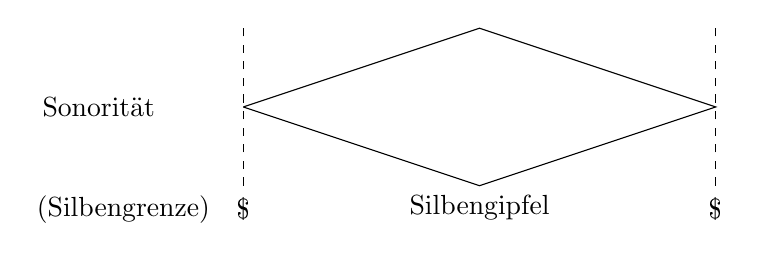
\begin{tikzpicture}
	\draw[dashed] (-3,0)--(-3,2);
	\draw[dashed] (3,0)--(3,2);
	\draw[black] (-3,1)--(0,2)--(3,1)--(0,0)--(-3,1);
	\node at (-3,-0.3){\$};
	\node at (3,-0.3){\$};
	\node[left] at (-3.3,-0.3){(Silbengrenze)};
	\node[left] at (-4,1){Sonorität};
	\node[below] at (0,0){Silbengipfel};
	\end{tikzpicture}
	\caption{Sonoritätsskala in \citet[19]{Lenerz85a}} %\citet[93]{Ramers08a}
\end{figure}
% Vokale sind sonorste Elemente
% m > p
% s > p  (frikativ > plosiv)

\begin{itemize}
	\item Laute können nach der Sonoritätshierarchie auf einer Skala (nach ihrer \textbf{Sonorität}) angeordnet werden.
\end{itemize}

\end{frame}


%%%%%%%%%%%%%%%%%%%%%%%%%%%%%%%%%%
\begin{frame}
\frametitle{Varianten der Sonoritätshierarchie}

Es gibt verschiedene Ausformulierungen der Sonoritätshierachie.


\begin{table}
\centering
\begin{tabular}{l|l|l|l|l} 
	 & einfach 				  	 & Hall 					  & \textbf{Wiese} 				& komplex  \\ 
\hline
\hline 
$[+]$& \multirow{6}{*}{Sonorant} & \multirow{2}{*}{Vokal} 	  & \multirow{2}{*}{Vokal} 		& Vokal  \\ 
	 & 							 & 						 	  &								& Vokal (hoch) \\
\cline{3-5}			
	 &							 & \multirow{3}{*}{Liquide}   &								& Gleitlaut \\
	 &						  	 &	 						  & \textipa{/\textscr /}		& Vibrant \\
\cline{4-5}			
	 &						 	 &							  & \textipa{/l/}				& Lateral \\
\cline{3-5}			
	 &							 & Nasal					  & Nasal						& Nasal \\
\hline			
	 &\multirow{6}{*}{Obstruent} & \multirow{6}{*}{Obstruent} & \multirow{3}{*}{Frikativ}	& $[+$sth$]$ Frikativ \\
	 &						 	 &							  &								& $[+$sth$]$ Affrikat \\		
	 &							 &							  &								& $[+$sth$]$ Plosiv \\
\cline{4-5}			
	 &						  	 &							  & \multirow{3}{*}{Plosiv}		& $[-$sth$]$ Frikativ \\
	 &						 	 &							  &								& $[-$sth$]$ Affrikat \\		
$[-]$&							 &							  &								& $[-$sth$]$ Plosiv \\
		
\end{tabular} 

\end{table}

\end{frame}



%%%%%%%%%%%%%%%%%%%%%%%%%%%%%%%%%%

\begin{frame}
%\frametitle{Sonoritätshierarchie}


\begin{block}{Sonoritätsprinzip (Sonority Sequencing Generalization -- SSG)}
In jeder Silbe gibt es ein Segment, das den \textbf{Silbengipfel} bildet, und dem ein oder mehrere Segmente vorangehen und/oder folgen, deren Sonoritätswerte \textbf{zum Silbengipfel hin zunehmen} und \textbf{danach abnehmen}.\\
\hfill (vgl. \citealt[225]{Hall00a}, \citealt[94]{Ramers08a})
\end{block}

\begin{itemize}
	\item Strikt: monoton steigend oder fallend
	\item Abgeschwächt: auch gleichbleibend \citep[vgl.][]{Hall00a}

\end{itemize}


\begin{figure}
	\centering
	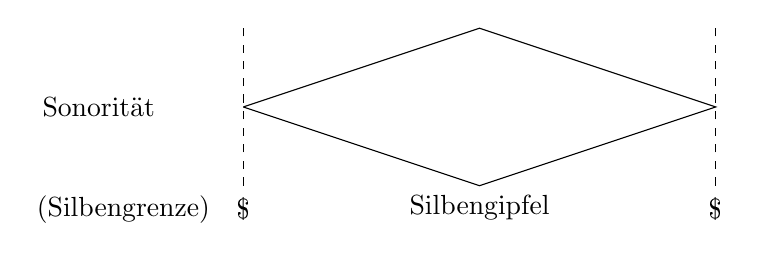
\begin{tikzpicture}
	\draw[dashed] (-3,0)--(-3,2);
	\draw[dashed] (3,0)--(3,2);
	\draw[black] (-3,1)--(0,2)--(3,1)--(0,0)--(-3,1);
	\node at (-3,-0.3){\$};
	\node at (3,-0.3){\$};
	\node[left] at (-3.3,-0.3){(Silbengrenze)};
	\node[left] at (-4,1){Sonorität};
	\node[below] at (0,0){Silbengipfel};
\end{tikzpicture}
	\caption{Sonoritätsskala in \citet[19]{Lenerz85a}} %\citet[93]{Ramers08a}
\end{figure}


\end{frame}


%%%%%%%%%%%%%%%%%%%%%%%%%%%%%%%%%%
\begin{frame}
%\frametitle{Sonoritätshierarchie}

\begin{block}{Sonoritätshierarchie (für uns)}
Vokal $>$ \textipa{/\textscr /} $>$ \textipa{/l/} $>$ Nasal $>$ Frikativ $>$ Plosiv \\
$x > y$ $:=$ $x$ ist sonorer als $y$
\end{block}

\begin{figure}
	\centering
	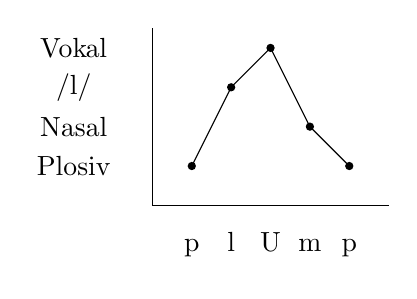
\begin{tikzpicture}[scale=0.5]
	\draw[black] (-1,0) -- (5,0) ; % x axis
	\draw[black] (-1,0) -- (-1,4.5); % y axis
	\node at (-3,1) {Plosiv};
	\node at (-3,2) {Nasal};
	\node at (-3,3) {\textipa{/l/}};
	\node at (-3,4) {Vokal};
	\draw[black] (0,1) -- (1,3) -- (2,4) -- (3,2) -- (4,1);
	\node at (0,-1) {\strut \textipa{p}};
	\node at (1,-1) {\strut \textipa{l}};
	\node at (2,-1) {\strut \textipa{U}};
	\node at (3,-1) {\strut \textipa{m}};
	\node at (4,-1) {\strut \textipa{p}};
	\fill (0,1) circle [radius=3pt];
	\fill (1,3) circle [radius=3pt];
	\fill (2,4) circle [radius=3pt];
	\fill (3,2) circle [radius=3pt];
	\fill (4,1) circle [radius=3pt];
	\end{tikzpicture}
\caption{\citep[225]{Hall00a}}
\end{figure}


%\begin{figure}
%\centering
%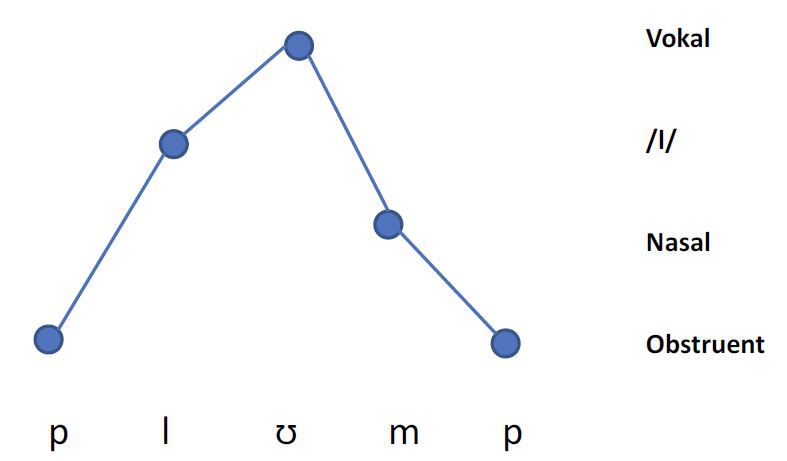
\includegraphics[scale=.3]{material/03bSonoritaetBsp}
%\caption{\citet[225]{Hall00a}}
%\end{figure}

\begin{itemize}
	\item Sonoritätshierarchie wird je nach Sprache leicht anders spezifiziert.
\end{itemize}
\end{frame}


%%%%%%%%%%%%%%%%%%%%%%%%%%%%%%%%%%
\begin{frame}
\frametitle{Übung}

\begin{itemize}
	\item Geben Sie die Sonoritätsprofile der folgenden Silben an.
	
	\ea Spatz, Dachs, Clown, Milch
	\z
	
	% bei Spatz geht es von Frikativ s auf Plosiv p runter = Ausnahme
	% bei Dachs geht es auf k runter und dann auf s hoch   = Ausnahme
	% clown k = plosiv, l = /l/ au = Vokal, n = , keine Ausnahme
	
	% Glottal stop gehört zu den Plosiven
	
	\item Erklären Sie die Ungrammatikalität der folgenden Silben:
	
	\begin{exe}
	\ex \label{ex:lbat}
	\begin{xlist}
		\ex [*]{\textipa{[lbat]}}
		\ex [*]{\textipa{[blabl]}}
		\ex [*]{\textipa{[ki:l\textscr]}}
		\ex [*]{\textipa{[ngang]}}
		\ex [*]{\textipa{[krafm]}}
		\ex [*]{\textipa{[elat]}}
		\ex [*]{\textipa{[plaml]}}
		\ex [*]{\textipa{[nfatl]}}
	\end{xlist}
\end{exe}
	
\end{itemize}

\end{frame}


%%%%%%%%%%%%%%%%%%%%%%%%%%%%%%%%%%%
\iftoggle{ue-loesung}{
	%%%%%%%%%%%%%%%%%%%%%%%%%%%%%%%%%%
%% UE 1 - 03b Phonologie
%%%%%%%%%%%%%%%%%%%%%%%%%%%%%%%%%%

\begin{frame}
\frametitle{Übung: Sonoritätsprofile -- Lösung}

\vfill
\hfill
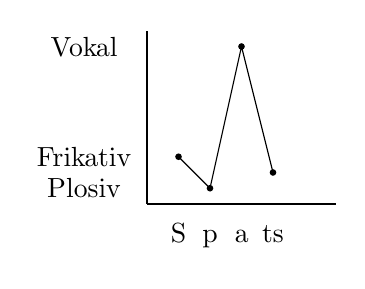
\begin{tikzpicture}[scale=0.4]
\draw[black] (-1,0) -- (5,0) ; % x axis
\draw[black] (-1,0) -- (-1,5.5); % y axis
\node at (-3,0.5) {Plosiv};
\node at (-3,1.5) {Frikativ};
\node at (-3,5) {Vokal};
\draw[black] (0,1.5) -- (1,0.5) -- (2,5) -- (3,1);
\node at (0,-1) {\strut \textipa{S}};
\node at (1,-1) {\strut \textipa{p}};
\node at (2,-1) {\strut \textipa{a}};
\node at (3,-1) {\strut \textipa{\texttoptiebar{ts}}};
\fill (0,1.5) circle [radius=3pt];
\fill (1,0.5) circle [radius=3pt];
\fill (2,5) circle [radius=3pt];
\fill (3,1) circle [radius=3pt];
\end{tikzpicture}
\pause
\hfill
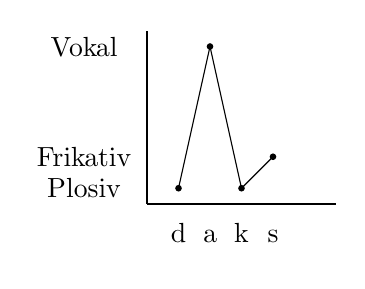
\begin{tikzpicture}[scale=0.4]
\draw[black] (-1,0) -- (5,0) ; % x axis
\draw[black] (-1,0) -- (-1,5.5); % y axis
\node at (-3,0.5) {Plosiv};
\node at (-3,1.5) {Frikativ};
\node at (-3,5) {Vokal};
\draw[black] (0,0.5) -- (1,5) -- (2,0.5) -- (3,1.5);
\node at (0,-1) {\strut \textipa{d}};
\node at (1,-1) {\strut \textipa{a}};
\node at (2,-1) {\strut \textipa{k}};
\node at (3,-1) {\strut \textipa{s}};
\fill (0,0.5) circle [radius=3pt];
\fill (1,5) circle [radius=3pt];
\fill (2,0.5) circle [radius=3pt];
\fill (3,1.5) circle [radius=3pt];
\end{tikzpicture}
\hfill\mbox{}
\vfill
\pause
\hfill
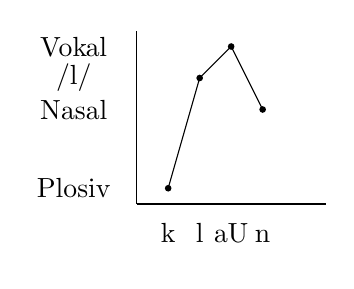
\begin{tikzpicture}[scale=0.4]
\draw[black] (-1,0) -- (5,0) ; % x axis
\draw[black] (-1,0) -- (-1,5.5); % y axis
\node at (-3,0.5) {Plosiv};
\node at (-3,3) {Nasal};
\node at (-3,4) {\textipa{/l/}};
\node at (-3,5) {Vokal};
\draw[black] (0,0.5) -- (1,4) -- (2,5) -- (3,3);
\node at (0,-1) {\strut \textipa{k}};
\node at (1,-1) {\strut \textipa{l}};
\node at (2,-1) {\strut \textipa{\texttoptiebar{aU}}};
\node at (3,-1) {\strut \textipa{n}};
\fill (0,0.5) circle [radius=3pt];
\fill (1,4) circle [radius=3pt];
\fill (2,5) circle [radius=3pt];
\fill (3,3) circle [radius=3pt];
\end{tikzpicture}
\hfill
\pause
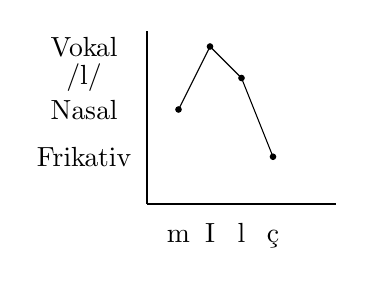
\begin{tikzpicture}[scale=0.4]
\draw[black] (-1,0) -- (5,0) ; % x axis
\draw[black] (-1,0) -- (-1,5.5); % y axis
\node at (-3,1.5) {Frikativ};
\node at (-3,3) {Nasal};
\node at (-3,4) {\textipa{/l/}};
\node at (-3,5) {Vokal};
\draw[black] (0,3) -- (1,5) -- (2,4) -- (3,1.5);
\node at (0,-1) {\strut \textipa{m}};
\node at (1,-1) {\strut \textipa{I}};
\node at (2,-1) {\strut \textipa{l}};
\node at (3,-1) {\strut \textipa{\c{c}}};
\fill (0,3) circle [radius=3pt];
\fill (1,5) circle [radius=3pt];
\fill (2,4) circle [radius=3pt];
\fill (3,1.5) circle [radius=3pt];
\end{tikzpicture}
\hfill\mbox{}
\vfill
\end{frame}


%%%%%%%%%%%%%%%%%%%%%%%%%%%%%%%%%%
\begin{frame}
\frametitle{Übung -- Lösung}

\begin{itemize}
\item Erklären Sie die Ungrammatikalität der folgenden Silben:\\
(Vokal $>$ \textipa{/\textscr /} $>$ \textipa{/l/} $>$ Nasal $>$ Frikativ $>$ Plosiv)
\begin{exe}
	\exr{ex:lbat}
	\settowidth\jamwidth{XXXXXXXXXXXXXXXXXXXXXXXXXXXXXXXXXX}
	\begin{xlist}
		\ex[*]{ \textipa{[lbat]}\loesung{2}{\textipa{[l]} vor \textipa{[b]} im Onset} }
		\ex[*]{ \textipa{[blabl]}\loesung{3}{\textipa{[b]} vor \textipa{[l]} in der Koda $+$ Auslautverhärtung} }
		\ex[*]{ \textipa{[{\textscr}mapt]}\loesung{4}{\textipa{[\textscr ]}vor \textipa{[m]} im Onset } }
		\ex[*]{ \textipa{[ki:l\textscr]}\loesung{5}{\textipa{[l]} vor \textipa{[\textscr ]} in der Koda} }
		\ex[*]{ \textipa{[ngang]}\loesung{6}{\textipa{[n]} vor \textipa{[g]} im Onset $+$ reg. velare Nasalassimiliation } \loesung{6}{$+$ g-Tilgung}}
		\ex[*]{ \textipa{[krafm]}\loesung{7}{\textipa{[f]} vor \textipa{[m]} in der Koda} }
		\ex[*]{ \textipa{[elat]}\loesung{8}{2 Silben (2 Nuklei) $+$ Knacklauteinsetzung} }
		\ex[*]{ \textipa{[plaml]}\loesung{9}{\textipa{[m]} vor \textipa{[l]} in der Koda} }
		\ex[*]{ \textipa{[nfatl]}\loesung{10}{\textipa{[n]} vor \textipa{[f]} im Onset $+$ \textipa{[t]} vor \textipa{[l]} in der Koda} }
	\end{xlist}
\end{exe}

\end{itemize}

\end{frame}


}
%%%%%%%%%%%%%%%%%%%%%%%%%%%%%%%%%%

\subsubsection{Weitere phonotaktische Beschränkungen}

%%%%%%%%%%%%%%%%%%%%%%%%%%%%%%%%%%

\begin{frame}
\frametitle{Weitere phonotaktische Beschränkungen}

\begin{columns}
	
	\column{.6\textwidth}	
\begin{itemize}
	\item Im \textbf{Onset} in deutschen Silben können stehen:
	
	\begin{itemize}
		\item alle Einzelkonsonanten des Deutschen 
		
		(\textbf{außer} \textipa{[N]} und \textipa{[s]} vor Vokal am Wortanfang)

		\item bestimmte zwei- und dreigliedrige Konsonantencluster nach Sonoritätshierarchie
		
		\item bestimmte zweigliedrige Konsonantencluster\\
		 (s. Tabelle: von links nach oben im Onset, in der Koda umgekehrt, \citealp[vgl.][231-235]{Hall00a})
	\end{itemize}

	\ea *\textipa{[fma]} \vs \textipa{[fla]}
	\ex *\textipa{[lpa]} \vs \textipa{[pla]}
	\ex *\textipa{[mSa]} \vs \textipa{[Sma]}
	\ex *\textipa{[m\;Ra]}
	\z
\end{itemize}
	
	\column{.35\textwidth}
\begin{table}
	\centering
	
	\begin{tabular}{c|c|c|c|c}
		& \textipa{m} & \textipa{n} & \textipa{l} & \textipa{\textscr} \\ 
		\hline 
		\textipa{p} &  &  & $+$ & $+$ \\ 
		\hline 
		\textipa{b} &  &  & $+$ & $+$ \\ 
		\hline 
		\textipa{t} &  &  &  & $+$ \\ 
		\hline 
		\textipa{d} &  &  &  & $+$ \\ 
		\hline 
		\textipa{k} &  & $+$ & $+$ & $+$ \\ 
		\hline 
		\textipa{g} &  & $+$ & $+$ & $+$ \\ 
		\hline 
		\textipa{f} &  &  & $+$ & $+$ \\
		\hline 
		\textipa{v} &  &  &  & $+$ \\ 
		\hline 
		\textipa{S} & $+$ & $+$ & $+$ & $+$ \\ 
	\end{tabular} 
	
	\caption{Kombinatorik von Sonoranten mit Obstruenten im Deutschen}
\end{table}

\end{columns}	

\end{frame}	
%%%%%%%%%%%%%%%%%%%%%%%%%%%%%%%%%

\begin{frame}{Weitere phonotaktische Beschränkungen}
	
\begin{itemize}	
	\item Silben können auch \textbf{mit unbetontem Vokal} beginnen (\ras leerer Onset).
	\ea \ab{Eier}: \textipa{[\textprimstress P\t{aɪ}.\alertred{5}]}
	\z
	
	\ea \ab{etwaig}: \textipa{[PEt.\textprimstress va:.\alertred{I}\c{c}]} 
	\z

\pause 
	
	\item Vor betontem Vokal steht immer ein Konsonant (\textbf{Glottisschlag}).
	
	\ea
	\textipa{[ka.\alertred{\textprimstress Po:}.tIS]}
	\z

\end{itemize}

\end{frame}


%%%%%%%%%%%%%%%%%%%%%%%%%%%%%%%%%%
\subsection{Hausaufgabe}
%%%%%%%%%%%%%%%%%%%%%%%%%%%%%%%%%%

\begin{frame}
\frametitle{Hausaufgabe}

\begin{itemize}
	\item[1.]{Geben Sie die standarddeutsche \textbf{phonetische Transkription} für folgende Wörter an:}
	
	\eal \label{ex:03bHA1}
	\ex Spitzenschuhe
	\ex Endausscheidung
	\ex Platzanweiser
	\ex verzweifeln
	\ex abverlangen
	\ex Überarbeitung
	\ex Zugeständnis
	\zl
\end{itemize}

\end{frame}
%%%%%%%%%%%%%%%%%%%%%%%%%%%%%%%%%

\begin{frame}{Hausaufgabe}

\begin{itemize}
\item[2.]{Erläutern Sie anhand der folgenden Beispiele, unter welchen Bedingungen die \textbf{Auslautverhärtung} im Deutschen stattfindet.}

\eal \label{ex:03bHA2}
\ex Wand -- Wände
\ex lesen -- lesbar
\ex sagen -- sagst
\ex Roggen
\exi{}{Für Fortgeschrittene auch noch:}
\ex schnell gesprochenes \textit{hab' ich}
\zl

\end{itemize}

\end{frame}
%%%%%%%%%%%%%%%%%%%%%%%%%%%%%%%%%%

\begin{frame}{Hausaufgabe}

\begin{itemize}
\item[3.]{Geben Sie fünf verschiedene \textbf{phonetische oder phonologische Prozesse} an, die in dem folgenden Satz -- teilweise nur bei schnellerem Sprechen -- beobachtet werden können.} 

\ea \label{ex:03bHA3}
\begin{quote}
Um die fünf Haken in regelmäßigen Abständen an die Wand schrauben zu können, sollten Sie sich Bohrmaschine, Wasserwaage, Zollstock und Dübel bereitgelegt haben und auf keinen Fall die Nerven verlieren, bevor Sie nicht befestigt sind.
\end{quote}
\z

\end{itemize}

\end{frame}
%%%%%%%%%%%%%%%%%%%%%%%%%%%%%%%%%%%

\begin{frame}{Hausaufgabe}

\begin{itemize}	
\item[4.]{Illustrieren Sie den deutschen phonemischen Kontrast der folgenden Phoneme durch
  \textbf{Minimalpaare}, wobei der Kontrast (wenn möglich) ein Mal initial,\\
ein Mal final vorkommen soll.

Beispiel: \textipa{[p]} -- \textipa{[f]} Paul -- faul (Initialposition), Laub -- Lauf (Finalposition)}

\eal \label{ex:03bHA4}
\ex \textipa{[m]} -- \textipa{[n]}
\ex \textipa{[p]} -- \textipa{[b]}
\ex \textipa{[h]} -- \textipa{[v]}
\ex \textipa{[n]} -- \textipa{[N]}
\ex \textipa{[f]} -- \textipa{[v]}
\zl

\end{itemize}
\end{frame}


%%%%%%%%%%%%%%%%%%%%%%%%%%%%%%%%%%%
\iftoggle{ha-loesung}{
	%%%%%%%%%%%%%%%%%%%%%%%%%%%%%%%%%%
%% HA 1 - 03b Phonologie
%%%%%%%%%%%%%%%%%%%%%%%%%%%%%%%%%%

\begin{frame}
\frametitle{Hausaufgabe -- Lösung}

\begin{itemize}
	\item[1.]{Geben Sie die standarddeutsche \textbf{phonetische Transkription} für folgende Wörter an:}
	
	\begin{exe}
		\exr{ex:03bHA1}
		\begin{xlist}
		\settowidth\jamwidth{XXXXXXXXXXXXXXXXXXXXXXXXXXXXXX}
			\ex Spitzenschuhe \loesung{2}{\textipa{['SpI\textsubdot{\t{ts}}@n.Su:.@]}}
			\ex Endausscheidung \loesung{3}{\textipa{['PEnt.P\texttoptiebar{aU}s.S\texttoptiebar{aI}.dUN]}}
			\ex Platzanweiser \loesung{4}{\textipa{['pla\texttoptiebar{ts}.Pan.v\texttoptiebar{aI}.z5]}}
			\ex verzweifeln \loesung{5}{\textipa{[fE5.'\texttoptiebar{ts}v\texttoptiebar{aI}.f@ln]}}
			\ex abverlangen \loesung{6}{\textipa{['Pap.fE5.la\.N@n]}}
			\ex Überarbeitung \loesung{7}{\textipa{[Py:.b5.'Pa\;R.b\texttoptiebar{aI}.tUN]}}
			\ex Zugeständnis \loesung{8}{\textipa{['\texttoptiebar{ts}u:.g@.StEnt.nIs]}}
		\end{xlist}
	\end{exe}

\end{itemize}

\end{frame}
%%%%%%%%%%%%%%%%%%%%%%%%%%%%%%%%%

\begin{frame}{Hausaufgabe -- Lösung}

\begin{itemize}
	\item[2.]{Erläutern Sie anhand der folgenden Beispiele, unter welchen Bedingungen die \textbf{Auslautverhärtung} im Deutschen stattfindet.}

	\begin{exe}
		\exr{ex:03bHA2}
		\begin{xlist}
		\settowidth\jamwidth{XXXXXXXXXXXXXXXXXXXXXXXXXXXXXXX}
			\ex Wand -- Wände \loesung{2}{sth. Plosive am Wortende}
			\ex lesen -- lesbar \loesung{3}{generell am Silbenende}
			\ex sagen -- sagst \loesung{4}{betrifft \emph{alle} sth. Plosive in der Koda}
			\ex Roggen \loesung{5}{jedoch keine Silbengelenke}
		\end{xlist}
	\end{exe}

\end{itemize}

\end{frame}


%%%%%%%%%%%%%%%%%%%%%%%%%%%%%%%%%%
\begin{frame}{Hausaufgabe -- Lösung}

\begin{itemize}
\item[3.]{Geben Sie fünf verschiedene \textbf{phonetische oder phonologische Prozesse} an, die in dem folgenden Satz -- teilweise nur bei schnellerem Sprechen -- beobachtet werden können.} 

\begin{exe}
	\exr{ex:03bHA3}
	\begin{quote}
	Um die fünf Haken in regelmäßigen Abständen an die Wand schrauben zu können, sollten Sie sich Bohrmaschine, Wasserwaage, Zollstock und Dübel bereitgelegt haben und auf keinen Fall die Nerven verlieren, bevor Sie nicht befestigt sind.
	\end{quote}
\end{exe}


\begin{description}
	\item[\alertgreen{\textbf{Beispiele:}}] ~

\alertgreen{
	regressive Nasalassimilation in \emph{fünf}: \textipa{[fY\textbf{m}f]}\\
	progressive Nasalassimilation nach Schwa-Elision (feeding) in \emph{Haken}: \textipa{[hak\textbf{N}]}\\
	Auslautverhärtung in \emph{Wand}: \textipa{[van\textbf{t}]}\\
	progressive Nasalassimilation nach Schwa-Elision (feeding) in \emph{schrauben}: \textipa{[S\;R\t{aU}b\textbf{m}]}\\
	g-Spirantisierung in \emph{befestigt}: \textipa{[b@fEstI\textbf{\c{c}}t]}\\
	r-Vokalisierung in \emph{Bohrmaschine}: \textipa{[bo\textbf{5}maSi:n@]}
}						
		\end{description}

\end{itemize}

\end{frame}


%%%%%%%%%%%%%%%%%%%%%%%%%%%%%%%%%%%
\begin{frame}{Hausaufgabe -- Lösung}

\begin{itemize}	
\item[4.]{Illustrieren Sie den deutschen phonemischen Kontrast der folgenden Phoneme durch \textbf{Minimalpaare}, wobei der Kontrast (wenn möglich) ein Mal initial, ein Mal final vorkommen soll.

Beispiel: \textipa{[p]} -- \textipa{[f]} Paul -- faul (Initialposition), Laub -- Lauf (Finalposition)}

\begin{exe}
	\exr{ex:03bHA4}
	\settowidth\jamwidth{XXXXXXXXXXXXXXXXXXXXXXXXXXXXXXXXXXXX}
	\begin{xlist}
		\ex \textipa{[m]} -- \textipa{[n]} \loesung{2}{muss -- Nuss, beim -- Bein}
		\ex \textipa{[p]} -- \textipa{[b]} \loesung{3}{Pass -- Bass}
			\loesung{3}{(wegen Auslautverhärtung kein finaler Kontrast möglich)}
		\ex \textipa{[h]} -- \textipa{[v]} \loesung{4}{heiß -- weiß (\textipa{[h]} kommt nicht final vor)}
		\ex \textipa{[n]} -- \textipa{[N]} \loesung{5}{Sinn -- sing (\textipa{[N]} kommt nicht initial vor)}
		\ex \textipa{[f]} -- \textipa{[v]} \loesung{6}{Fass -- was}
			\loesung{6}{(wegen Auslautverhärtung kein finaler Kontrast möglich)}
	\end{xlist}
\end{exe}
		
\end{itemize}

\end{frame}
}
%%%%%%%%%%%%%%%%%%%%%%%%%%%%%




%@EE: Checken: Keine Abbildungen und elektronischen Quellen?

